%%%
% File: /latex/big-cocluster-paper/sections/introduction.tex
% Created Date: Thursday, July 11th 2024
% Author: Zihan
% -----
% Last Modified: Sunday, 14th July 2024 9:44:18 pm
% Modified By: the developer formerly known as Zihan at <wzh4464@gmail.com>
% -----
% HISTORY:
% Date      		By   	Comments
% ----------		------	---------------------------------------------------------
%%%

\section{Introduction}
Artificial Intelligence is a rapidly advancing technology facilitating complex data analysis, pattern recognition, and decision-making processes. Clustering, a fundamental unsupervised learning technique, groups data points based on shared features, aiding in interpreting complex data structures. However, traditional clustering algorithms \cite{zhang2023AdaptiveGraphConvolution, wu2023EffectiveClusteringStructured} treat all features of data uniformly and solely cluster either rows (samples) or columns (features),  as shown in Figure \ref{fig:cluster}. They oversimplified interpretations and overlooked critical context-specific relationships within the data, especially when dealing with large, high-dimensional datasets \cite{chen2023FastFlexibleBipartite, zhao2023MultiviewCoclusteringMultisimilarity, kumar2023CoclusteringBasedMethods}.

\textit{Co-clustering} \cite{kluger2003SpectralBiclusteringMicroarray, yan2017CoclusteringMultidimensionalBig} is a technique that groups rows (samples) and columns (features) simultaneously, as shown in Figure \ref{fig:cocluster}. It can reveal complex correlations between two different data types and is transformative in scenarios where the relationships between rows and columns are as important as the individual entities themselves. For example, in bioinformatics, co-clustering could identify gene-related patterns leading to biological insights by concurrently analyzing genes and conditions \cite{higham2007SpectralClusteringIts, kluger2003SpectralBiclusteringMicroarray, zhao2012BiclusteringAnalysisPattern}. In recommendation systems, co-clustering can simultaneously discover more fine-grained relationships between users and projects \cite{dhillon2007WeightedGraphCuts, chen2023ParallelNonNegativeMatrix}. Co-clustering extends traditional clustering methods, enhancing accuracy in pattern detection and broadening the scope of analyses.

\begin{figure}[htbp]
    \centering
    \begin{subfigure}[b]{0.22\textwidth}
        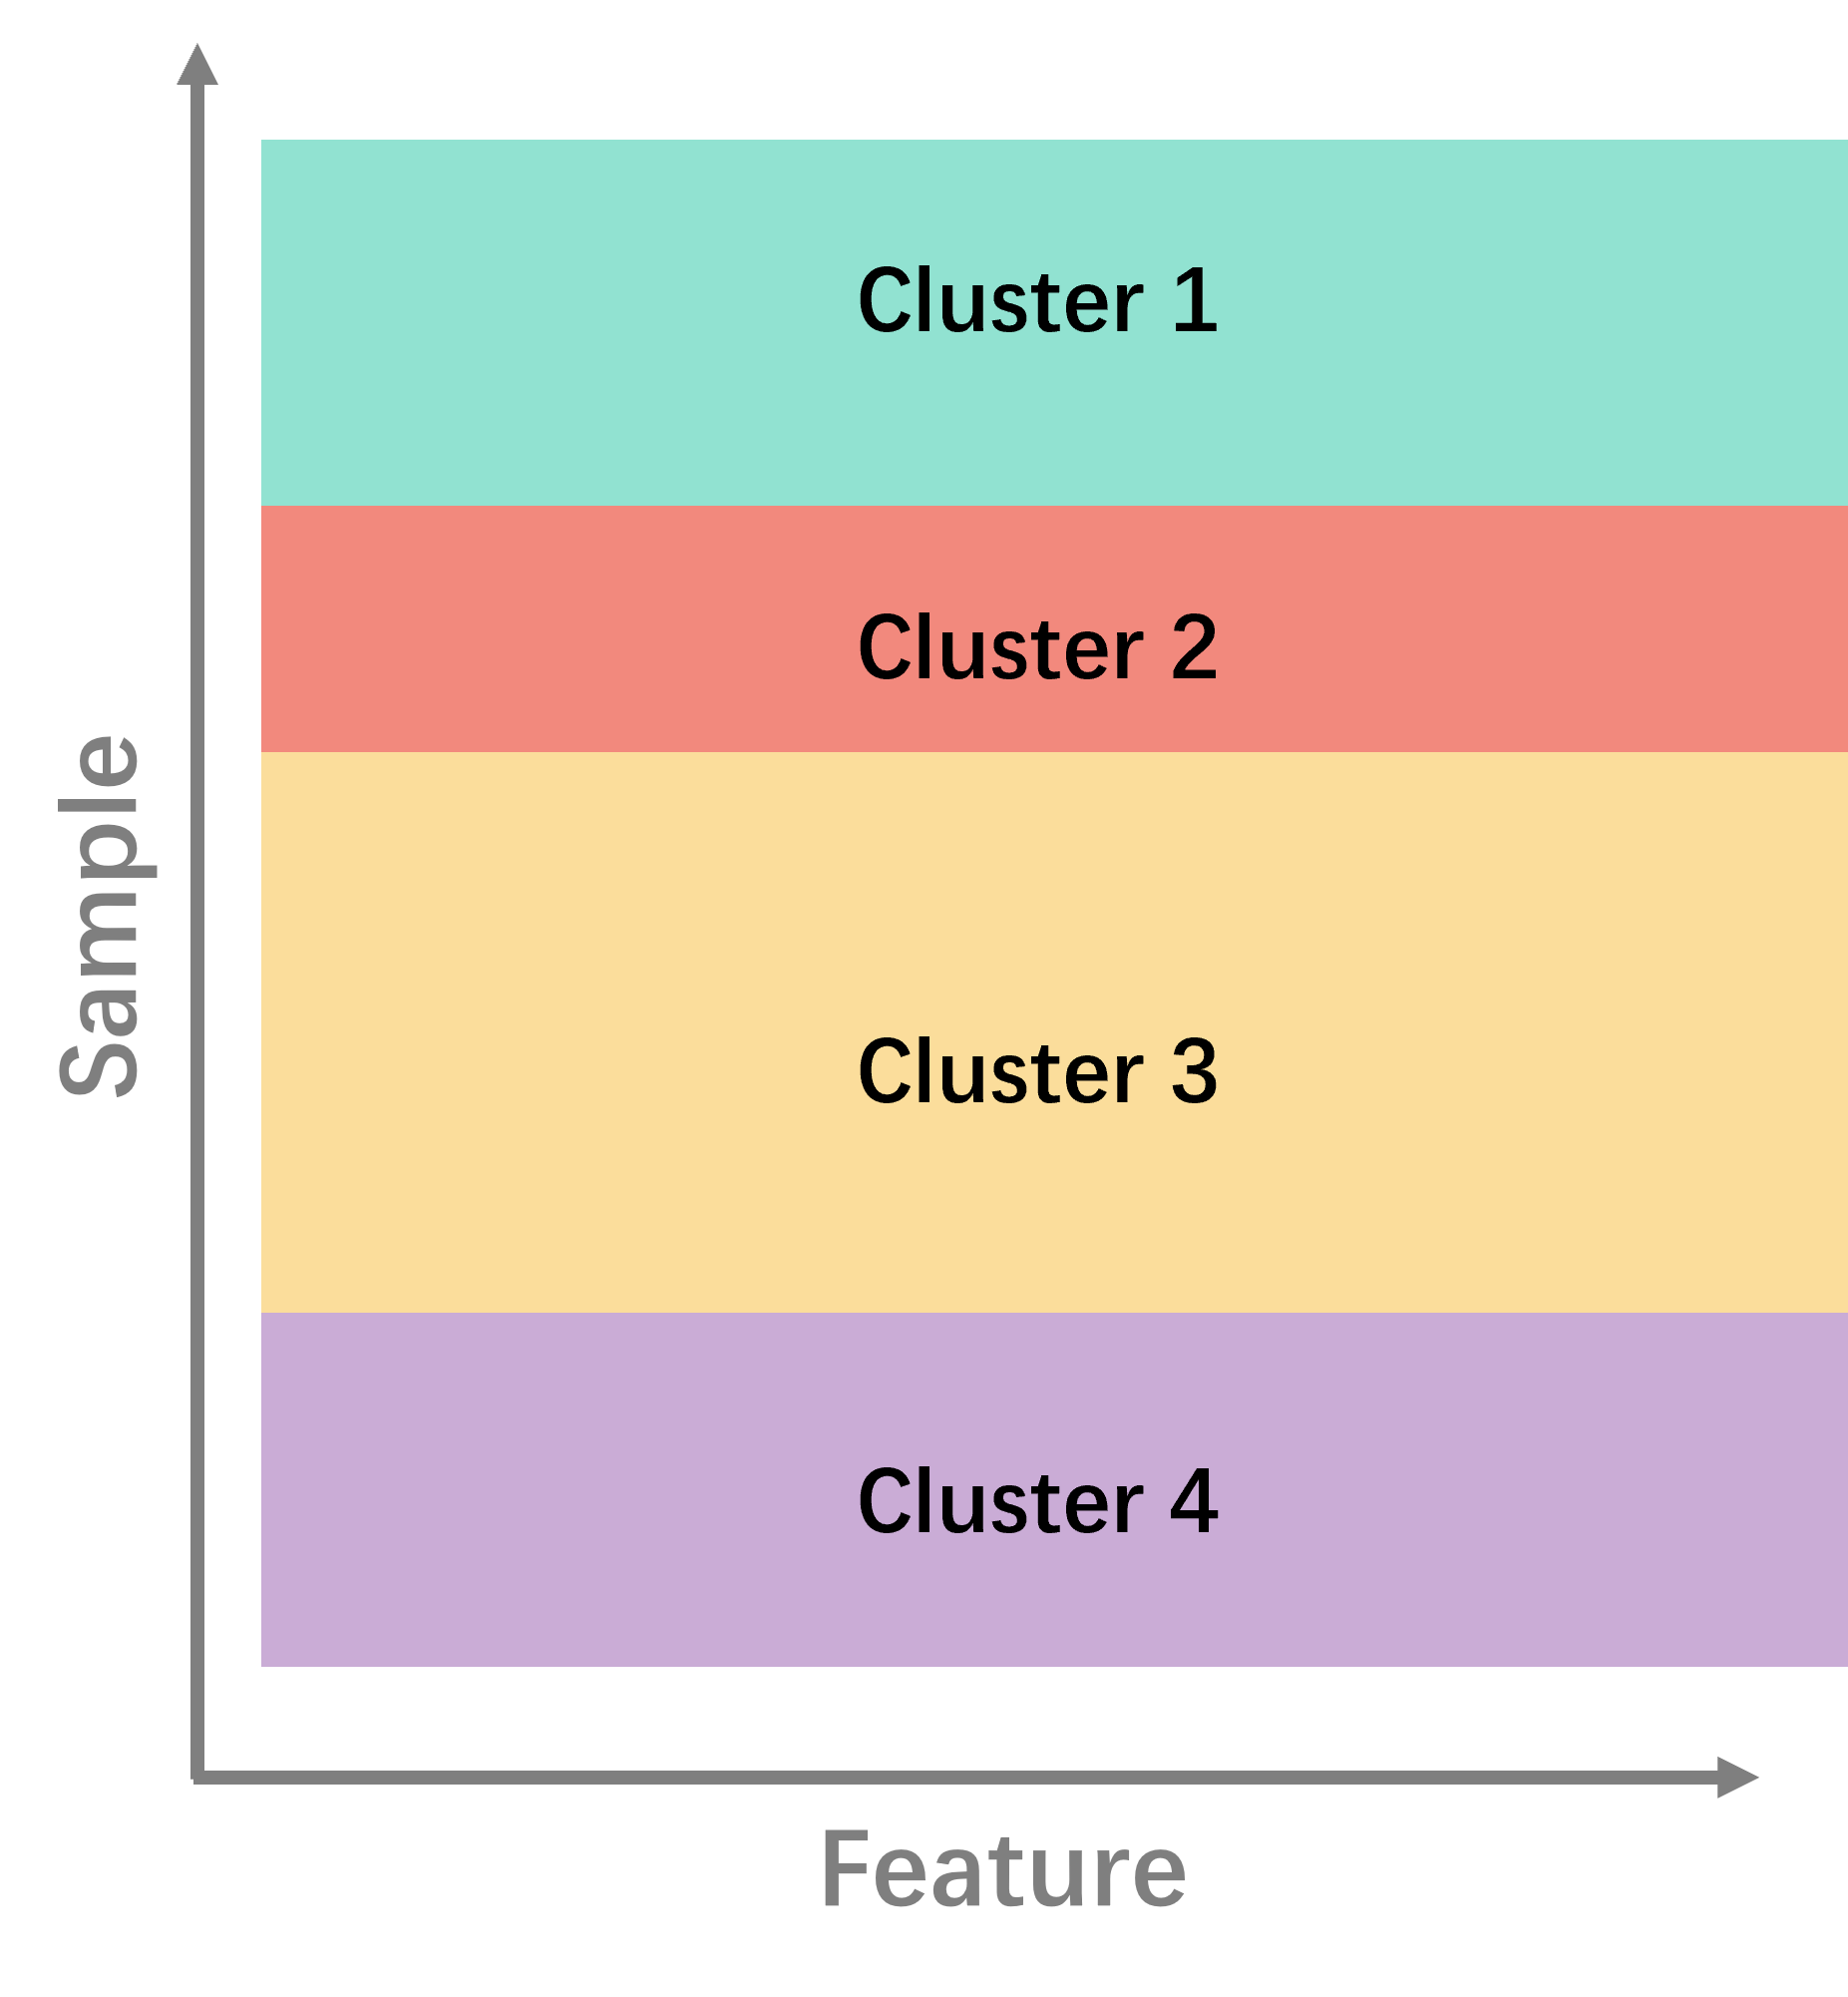
\includegraphics[width=\linewidth]{cluster.png}
        \caption{Clustering}
        \label{fig:cluster}
    \end{subfigure}
    \hfill
    \begin{subfigure}[b]{0.22\textwidth}
        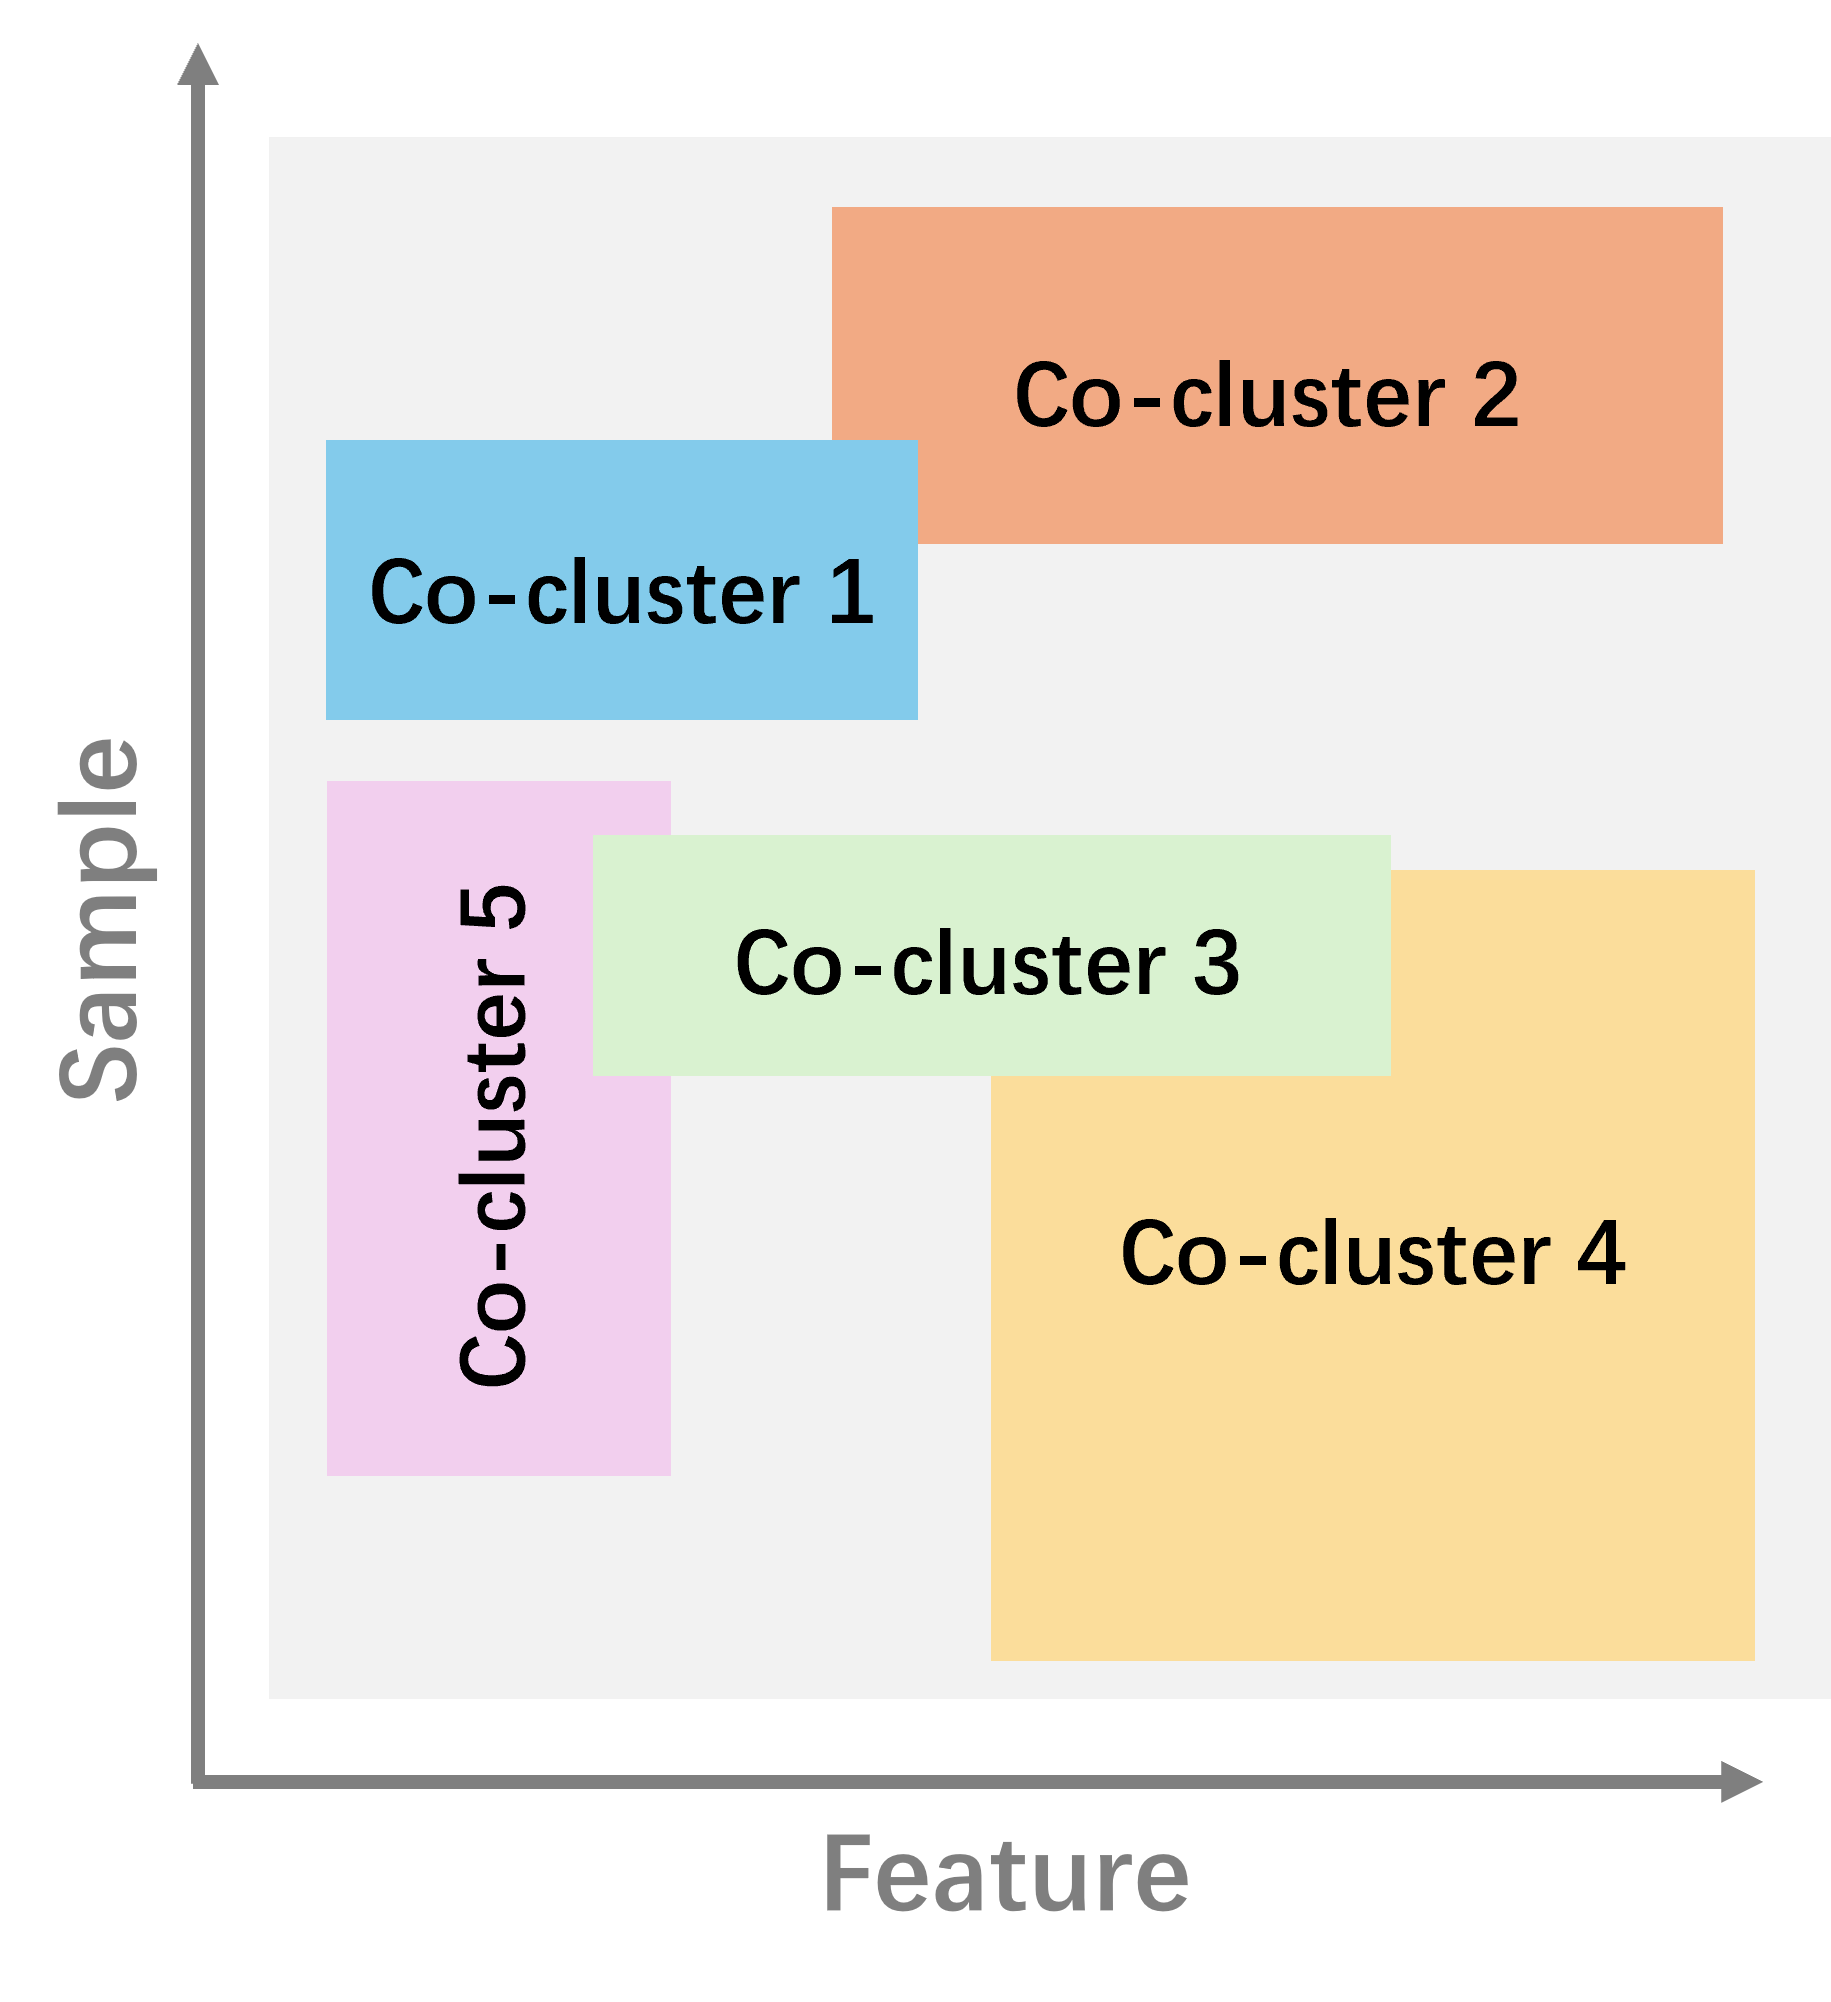
\includegraphics[width=\linewidth]{coc.png}
        \caption{Co-clustering}
        \label{fig:cocluster}
    \end{subfigure}
    \caption{An illustration of the differences between (a) Clustering and (b) Co-clustering \cite{yan2017CoclusteringMultidimensionalBig}.}
    \label{fig:cocomparison}
\end{figure}

Despite its potential, scaling co-clustering to large datasets poses significant challenges:

\begin{itemize}
    \item{\textbf{High Computational Complexity.}} Co-clustering analyzes relationships both within and across the rows and columns of a dataset simultaneously. This dual-focus analysis requires evaluating a vast number of potential relationships, particularly as the dimensions of the data increase. The complexity can grow exponentially with the size of the data because the algorithm must process every possible combination of rows and columns to identify meaningful clusters \cite{hansen2011NonparametricCoclusteringLarge}.
    \item{\textbf{Significant Communication Overhead.}} Even when methods such as data partitioning are used to handle large-scale data, each partition may independently analyze a subset of the data. However, to optimize the clustering results globally, these partitions need to exchange intermediate results frequently. This requirement is inherent to iterative optimization techniques used in co-clustering, where each iteration aims to refine the clusters based on new data insights, necessitating continuous updates across the network. Such extensive communication can become a bottleneck, significantly slowing down the overall processing speed.
    \item{\textbf{Dependency on Sparse Matrices.}} Several traditional co-clustering algorithms are designed to perform best with sparse matrices \cite{pan2008CRDFastCoclustering}. However, in many real-world applications, data matrices are often dense, meaning most elements are non-zero. Such scenarios present a significant challenge for standard co-clustering algorithms, as they must handle a larger volume of data without the computational shortcuts available with sparse matrices.
\end{itemize}

To address the inherent challenges associated with existing co-clustering methods, we propose a novel and scalable Adaptive Hierarchical Partitioning and Merging for Scalable Co-Clustering (\textbf{AHPM}) framework designed for large-scale datasets. First,  we propose a large matrix partitioning algorithm that divides the original data matrix into smaller submatrices. This partitioning facilitates parallel processing of co-clustering tasks across submatrices, significantly reducing both processing time and computational and storage demands for each processing unit. We also design a probabilistic model to determine the optimal number and configuration of these submatrices to ensure comprehensive data coverage.
Second, we develop a hierarchical co-cluster merging algorithm that iteratively combines the co-clusters from these submatrices. This process enhances the accuracy and reliability of the final co-clustering results and ensures robust and consistent clustering performance, particularly addressing issues of heterogeneity and model uncertainty.

The contributions of this paper are summarized as follows:
\begin{enumerate}
    \item \textbf{Large Matrix Partitioning Algorithm:}
          We propose a novel matrix partitioning algorithm that enables parallel co-clustering by dividing a large matrix into optimally configured submatrices. This design is supported by a probabilistic model that calculates the optimal number and order of submatrices, balancing computational efficiency with the detection of relevant co-clusters.
    \item \textbf{Hierarchical Co-cluster Merging Algorithm:}
          We design a hierarchical co-cluster merging algorithm that combines co-clusters from submatrices, ensuring the completion of the co-clustering process within a pre-fixed number of iterations. This algorithm significantly enhances the robustness and reliability of the co-clustering process, effectively addressing model uncertainty.
    \item \textbf{Experimental Valuation:}
          We evaluate the effectiveness and efficiency of our method across a wide range of scenarios with large, complex data. Experimental results show an approximate 83\% decrease for dense matrices and up to 30\% for sparse matrices.
\end{enumerate}

The rest of this paper is organized as: Section \ref{sec:related_work} reviews related works; Section \ref{sec:formula} presents the problem formulation; Section \ref{sec:method} describes our AHPM method; Section \ref{sec:experiment} reports experimental results; and Section \ref{sec:conclude} concludes the paper.
